
\chapter{Application Description}

\section{Architecture}

The application uses a combination of Event Driven architecture and Request-Response architecture, making as much use as possible of Node JS's\cite{NODEJS} built in capabilities for handling multiple operations on a single thread using concurrency and asynchronous programming.

The application consists of multiple microservices. These microservices implement communication patterns like \textit{Request-Response} and \textit{Publish/Subscribe}. All microservice communication is done using message queues like RabbitMQ and BullMQ. While RabbitMQ offers great support for both Request-Response communication and Publish/Subscribe communication, I chose to use BullMQ for Publish/Subscribe. BullMQ uses Redis to queue messages and process them. By using Redis, BullMQ offers an easy way to schedule the times when a message is executed and implement retry policies. On the other hand, RabbitMQ is built upon AMQP (Advanced Message Queuing Protocol)\cite{AMQP}. This makes it possbile to pass messsages across an internal network and register handlers for these messages. 

Since this application is heavily focused on microservices, here is a short description for each one of them:
\begin{itemize}
    % \item Client - User interface, hosted on a server of its own.
    \item \textbf{Webserver Service} - Single HTTP server, tasked with serving the client application and providing HTTP routes for fetching data.
    \item \textbf{Authentication Service} - Service handling all authentication logic. This server is only accessible via RabbitMQ queues.
    \item \textbf{Core Service} - Service handling all reads and writes to the database. This server is accessbile via RabbitMQ queues.
    \item \textbf{Authorization Service} - Service handling authorization across the whole application. The application implements a RBAC (Role Based Access Control). Each request goes through this service before reaching the Core service. Only accessbile via RabbitMQ.
    \item \textbf{Uploader Service} - Service handling all file uploads. Since uploads are usually resource intensive tasks and can fail due to numerous reasons, this is a processor service using BullMQ.
    \item \textbf{Mail Service} - Service handling all emails sent. Sending emails is also a resource intensive task especially if sending to multiple users at the same tim. This is a processor service using BullMQ.
    \item \textbf{Websocket Server} - Server exposing only a websocket connection. This server is handling all of the chat features inside of the application, listening for notifications sent by clients, invoking the Core service for different writes (saves, updates) to the database, and dispatching a notification to the intended client.
    \item \textbf{Notification Server} - Server exposing a route for handling SSE (Server Sent Events). This server is the one handling in-app notifications. 
\end{itemize}

\section{Features}
The main features of the application are: a steady authentication, a live-chat for allowing students to study in groups and a file-sharing system for easily sharing study notes.

\subsection{Authentication}
The most important part of any web based application is the authentication. While developing the authentication system for my application, I followed OAuth2\cite{OAUTH2} standards. 

\textbf{Registration}: During registration, users submit their full name, email, password and a confirmation password. The system hashes the password with a strong algorithm (implemented using bcryptjs), creates a new user record marked as unverified, and generates a time-limited email verification token. The token is stored in the database and emailed, prompting users to confirm their address.

Endpoint: /auth/register

Method: POST

Request Body: JSON Object containing fullname, email, password and confirmation password.

Response: JSON Object containing a success message if the request was successful

\begin{figure}[H]
  \centering
  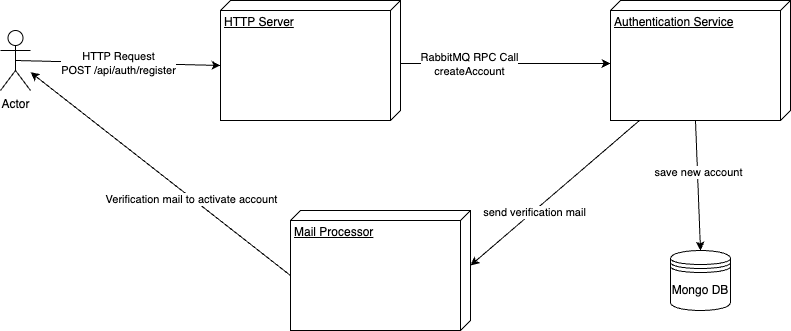
\includegraphics[width=1\linewidth]{licenta-register.drawio.png}
  \caption*{Register Flow}
  \label{fig:register-flow}
\end{figure}

\textbf{Verify Account}: When users click the verification link, the system extracts the token and searches the database for a matching, unexpired record. If valid, it marks the user’s account as verified, removes the token to prevent reuse, and returns a success response, enabling full access to login and other protected features.

Endpoint: /auth/verifyaccount

Method: GET

Query Parameters: verificationToken (string) -> verification token for certain account, recieved via email.

Response: JSON Object containing a success message if the request was successful


\textbf{Login}: On login, users submit credentials, which the system verifies against stored hashes. After confirming the account is verified, it generates a cryptographically secure session code, encrypts it, and stores it in the database under the user profile. The code is set in an HttpOnly, Secure cookie, establishing the authenticated session.

Endpoint: /auth/login

Method: POST

Request Body: JSON Object containing email, and password.

Response: JSON Object containing a success message if the request was successful.

\begin{figure}[H]
  \centering
  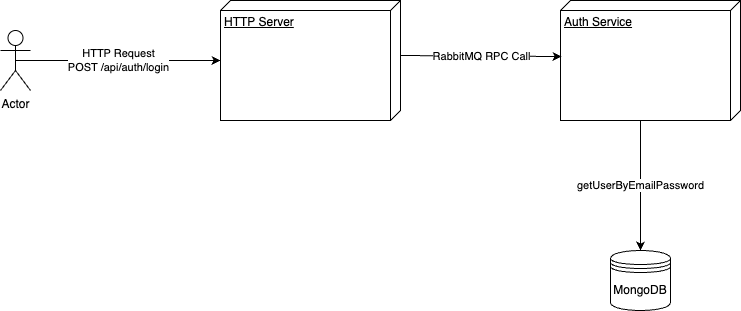
\includegraphics[width=1\linewidth]{licenta-login.drawio.png}
  \caption*{Login Flow}
  \label{fig:login-flow}
\end{figure}

\textbf{Reset Password}: When a password reset is requested, users provide their email address. The system generates a short-lived, cryptographically random reset token, stores it, and emails a reset link. Upon visiting the link and submitting a new password, the system validates the token, updates the password hash and deletes the token.

Endpoint: /auth/reset-password

Method: POST

Request Body: JSON Object containing reset token, password and confirmation password.

Response: JSON Object containing a success message if the request was successful


\textbf{Logout}: For logout, the client sends a request to invalidate the session. The server locates the encrypted session code in the database, removes it, and instructs the browser to clear the authentication cookie by setting it with a past expiration. The user is then unauthenticated for any subsequent requests.

Endpoint: /auth/logout

Method: POST

Response: JSON Object containing a success message if the request was successful.

\textbf{Whoami}: For Whoami, the client sends a request to get the user holding the current session. The server locates the encrypted session code in the database, and returns the user data.

Endpoint: /auth/whoami

Method: Get

Response: JSON Object containing userId, role and email of the logged in user if the request was successful.

\subsection{Live-chat}
The main part of any peer to peer platform is a real-time chat. Since this application focuses on providing students a way to communicate with each other in order to make stuying togheter easier, a real-time chat is a core functionality that I had to implement.

The real-time chat is implemented using Web Sockets\cite{WEB_SOCKET}. Even though Web Sockets are usually used for machine to machine communication, most applications that include a real-time chat like Microsoft Teams, Discord, Whatsapp use Web Sockets under to hood.

Web Sockets work by creating a bidirectional communication channel between clients and servers. Data is transported on this channel using messages. Each message must have a defined 'name' and maybe have some content.

In my implementation, I started by thinking about all of the messages that would be used inside of a chat application. After careful consideration, I ended up with 5 message types that my application must use:
\begin{itemize}
    \item \textbf{Join Conversation} - Message sent from the client side, containing the user authentication token and a conversationId. The server then checks if the user is a participant of that conversation, and responds back with a message of 'joined-conversation'.
    \begin{figure}[H]
        \centering
        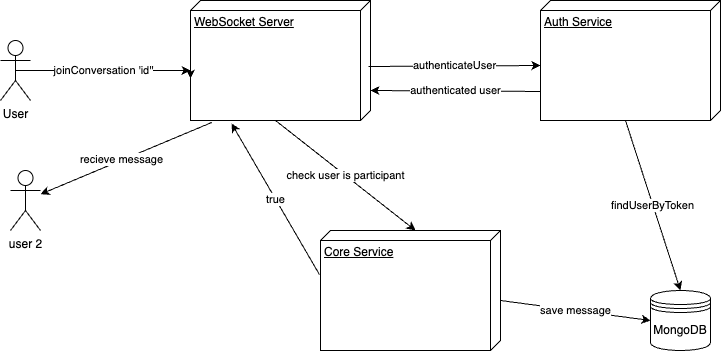
\includegraphics[width=1\linewidth]{licenta-join-conversation.drawio.png}
        \caption*{Join Conversation Flow}
        \label{fig:join-conversation-flow}
    \end{figure}
    \item \textbf{Leave Conversation} - This message is sent by the client side, when a user decides to leave a conversation. Leaving a conversation is done by either joining a different conversation, navigating to a different part of the application or closing the application. For this message, the server just removes the client from the conversation session.
    \item \textbf{Send Message} - This is the last and most importand message sent from the client application. Everytime the user creates a message and decides to send it, the application will send a message containing the user`s authentication token, message content and conversationId. After creating a database entry with the message details, the server responds back with 'recieve-message', in order to alret the application that a new message appeared.
    \begin{figure}[H]
        \centering
        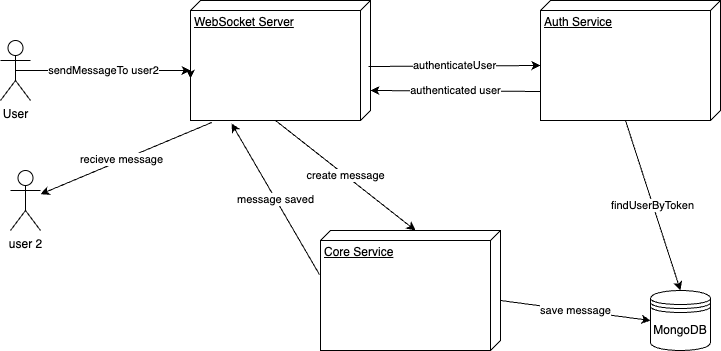
\includegraphics[width=1\linewidth]{licenta-ws.drawio.png}
        \caption*{Send Message Flow}
        \label{fig:send-message-flow}
    \end{figure}
    \item \textbf{Recieve Message} - The server sends this message after creating a entry in the database for the message sent by a user. The content of this message is the full database entry created. The client application listens for this message and correctly displays the new chat.
    \item \textbf{Joined Conversation} - After a user joins a conversation, the server sends this message back to the client application. This notifies the application that it can let the user start sending messages and recieving messages.
\end{itemize}

\subsection{File Uploader}
In the early days of file exchange, teams set up FTP servers on static IPs, juggling usernames, anonymous logins, and fragile directory hierarchies. Uploads would time out, backups were manual, and there was no easy way to integrate with modern web apps. As requirements grew—from embedding user-generated images in chat apps to serving large datasets via HTTP—FTP simply couldn’t keep up. Object storage emerged as the successor: a RESTful, scalable, self-healing store where applications can generate time-limited download links, automatically version files, and offload the burden of replication and durability. Today, replacing FTP with an S3-compatible store streamlines both developer workflows and end-user experience, turning clunky file drops into seamless, secure uploads and downloads.

S3-compatible object storage treats each file as an immutable “object” stored in a flat namespace of buckets. It exposes a simple HTTP API—PUT to upload, GET to download, DELETE to remove—so developers don’t wrestle with filesystem mounts or NFS quirks. Objects can carry arbitrary metadata (key/value tags or headers), and platforms often offer built-in features like automatic replication across nodes, lifecycle policies (e.g. archive or delete old versions), and fine-grained access controls. Because it’s designed for petabyte-scale data, S3-style stores provide high throughput for large payloads, seamless horizontal scaling, and durability guarantees that make them a natural fit for user uploads, backups, and any scenario where large binary blobs need reliable, cost-effective storage.

Traditional databases shine at structured records: rich querying, ACID transactions, indexing, and relationships across tables. However, stuffing multi-megabyte or multi-gigabyte files into a database can bloat its storage engine, slow down queries and backups, and drive up resource costs. In contrast, an S3-style object store offloads blob storage entirely, keeping the database lean for metadata lookups and relational joins. Object stores scale throughput linearly with added nodes, use pay-as-you-store pricing models, and excel at serving large downloads with built-in HTTP caching semantics. While a database might store a file’s URL and metadata, the object store holds the bytes—each in its own durable, self-healing container.

In \emph{Cloud Class}, the file uploader is a key component that allows users to share study materials, lecture notes, and other resources. It is designed to handle large files efficiently while ensuring reliability and scalability. The uploader integrates with an S3-compatible object storage service (MinIO) for storing files, and uses a message queue (BullMQ) to manage upload jobs asynchronously.

The file uploader is implemented as an asynchronous pipeline that delegates heavy I/O work to background workers. When a user submits a file, the client issues an HTTP POST to the webserver, which immediately enqueues a processing job and returns a 202 Accepted. A dedicated worker then uploads the file to object storage and notifies the persistence service to save metadata in the database, linking the file to the user’s record.

\begin{itemize}
\item \textbf{Client HTTP Request}
The frontend sends the file as \texttt{multipart/form-data} to \texttt{/files/upload} and receives back a job identifier.
\item \textbf{Webserver Endpoint}
The HTTP handler enqueues a “process-file” job on the queue, packaging the raw file bytes along with user context.
\item \textbf{Job Queue}
Redis + BullMQ persist and manage jobs with retry policies, ensuring uploads survive transient failures.
\item \textbf{Worker Process}
A background worker consumes each job, reconstructs the file buffer, generates a unique storage key, and uploads the file to the S3-compatible store.
\item \textbf{Object Storage}
Minio stores the binary in a bucket and returns a URL or object key.
\item \textbf{Persistence Service}
Upon successful storage, an event is sent to the core service, which creates a MongoDB document for the file (URL, key, MIME type, size, uploader ID, timestamps) and adds a reference to the user’s files array.
\end{itemize}

\begin{figure}[H]
\centering
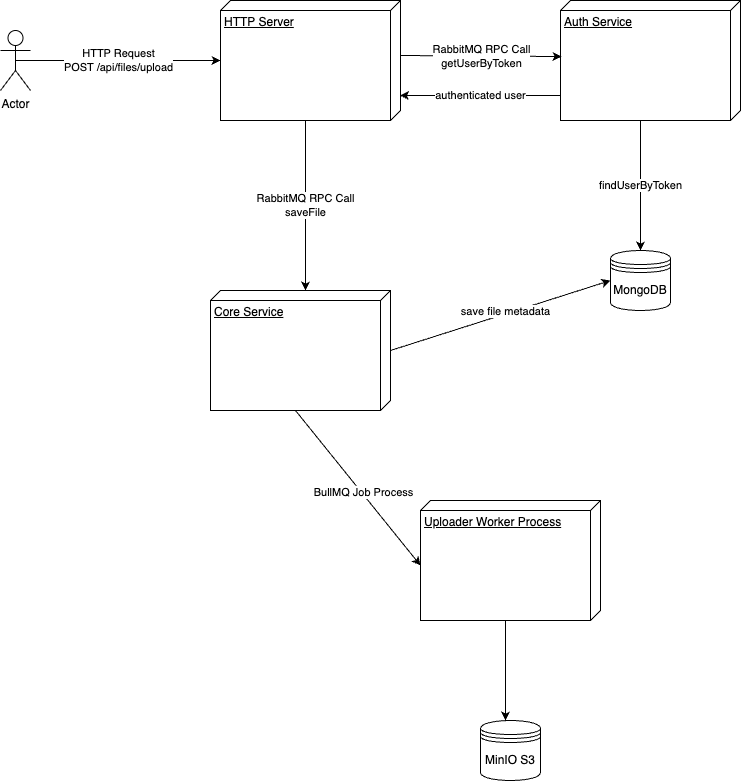
\includegraphics[width=1\linewidth]{licenta-uploader.drawio.png}
\caption*{File Upload Flow}
\label{fig:file-upload-flow}
\end{figure}

\section{Technology Stack}

The \emph{Cloud Class} application is a fully browser-based system built end-to-end in TypeScript/JavaScript.  Both client and server leverage modern, asynchronous architectures and microservices to ensure scalability, maintainability, and real-time interactivity.  This section outlines the key technologies and frameworks that form the backbone of our solution.

\subsection{Server Implementation}

The backend of \emph{Cloud Class} is implemented as a suite of modular microservices responsible for business logic, data persistence, and event handling.  All services are written in \mbox{TypeScript}, compiled to JavaScript, and orchestrated via Docker.

\begin{itemize}
  \item \textbf{TypeScript}  
    \begin{itemize}
      \item A statically typed superset of JavaScript that compiles to ES2019.  
      \item Enables interface-driven design, strong type checking, and advanced IDE support (e.g., IntelliSense).  
      \item Facilitates early detection of errors, consistent code formatting (TSLint / ESLint), and straightforward refactoring in large codebases.
    \end{itemize}

  \item \textbf{Node.js}  
    \begin{itemize}
      \item Event-driven, non-blocking I/O runtime built on Chrome’s V8 engine.  
      \item Ideal for handling high concurrency with minimal resource overhead.  
      \item Integrated with PM2 for process management, automatic restarts, and memory monitoring in production.
    \end{itemize}

  \item \textbf{NestJS}  
    \begin{itemize}
      \item Progressive Node.js framework leveraging decorators and dependency injection.  
      \item Promotes a modular architecture: controllers, providers, and gateways can be developed and tested independently.  
      \item Native support for REST, GraphQL, WebSockets, and microservice patterns (TCP, gRPC, Redis-based transport).
    \end{itemize}

  \item \textbf{MongoDB}  
    \begin{itemize}
      \item NoSQL document database storing data in flexible BSON format.  
      \item Supports horizontal scaling via sharding, automatic replica sets for high availability, and ACID transactions across multiple documents (v4.0+).  
      \item Optimized for rapid development cycles, enabling schema evolution without downtime.
    \end{itemize}

  \item \textbf{MinIO (S3-compatible)}  
    \begin{itemize}
      \item High-performance, Kubernetes-native object storage with Amazon S3 API compatibility.  
      \item Features erasure coding, bitrot protection, server-side encryption, and multi-tenant isolation.  
      \item Deployed as a StatefulSet in Kubernetes, ensuring persistent volumes and dynamic scaling.
    \end{itemize}

  \item \textbf{Real-Time Communication}  
    \begin{itemize}
      \item \emph{Socket.IO}: Bidirectional WebSocket library with automatic fallback to HTTP long-polling. Used for live chat, collaborative editing, and presence notifications.  
      \item \emph{Server-Sent Events (SSE)}: Lightweight, one-way event streams for broadcasting state changes (e.g., live class schedules, system alerts) with minimal overhead.
    \end{itemize}

  \item \textbf{Logging \& Analytics:}  
    \begin{itemize}
      \item \emph{Elasticsearch \& Kibana}: Distributed search and analytics engine powering full-text search, structured queries, and real-time log aggregation.  
      \item Logs are shipped via Filebeat into an ELK stack, enabling dashboards for performance monitoring, error tracking, and usage metrics.
    \end{itemize}

  \item \textbf{Testing}  
    \begin{itemize}
      \item \emph{Jest}: Zero-configuration JavaScript testing framework for unit and integration tests, featuring snapshot testing and code coverage reports.  
    \end{itemize}

  \item \textbf{Message Queues \& Background Jobs:}  
    \begin{itemize}
      \item \emph{RabbitMQ}: AMQP broker for reliable, complex routing of messages between microservices (e.g., task dispatch, order processing).  
      \item \emph{BullMQ}: Redis-backed job queue for scheduled and repeatable tasks such as email delivery, report generation, and notification bursts.  
      \item Combined to balance high-throughput event streams (RabbitMQ) with lightweight, retry-capable background jobs (BullMQ).
    \end{itemize}
\end{itemize}

\subsection{Client Implementation}

The frontend of \emph{Cloud Class} is a single-page application delivering responsive, component-driven user experiences.  Written in TypeScript and React, it communicates with backend microservices via REST, and real-time channels.

\begin{itemize}
  \item \textbf{HTML5 \& Semantic Markup}  
    \begin{itemize}
      \item Establishes the document structure with accessibility in mind (ARIA roles, landmarks).  
      \item Leveraged for SEO optimization, rich media embedding, and form-based user inputs (e.g., quizzes, surveys).
    \end{itemize}

  \item \textbf{CSS3 \& Responsive Design}  
    \begin{itemize}
      \item Utilizes Flexbox, Grid layouts, and custom properties (CSS variables) for adaptable, maintainable styling.  
      \item Media queries ensure seamless rendering across desktop, tablet, and mobile viewports.
    \end{itemize}

  \item \textbf{React \& TypeScript}  
    \begin{itemize}
      \item Component-based architecture with JSX syntax and a virtual DOM for efficient UI updates.  
    \end{itemize}

  \item \textbf{Real-Time Updates (Socket.IO Client)}  
    \begin{itemize}
      \item Establishes persistent WebSocket connections for instant notifications (e.g., new messages, collaborative whiteboard changes).  
      \item Automatic reconnection and event buffering ensure continuity during transient network issues.
    \end{itemize}
\end{itemize}

\section{Interface}
Present App interface using Screenshots?

Each figure has to have a caption that is a suggestive description of what  the  picture represents (e.g. Figure \ref{fig:siglaUVT}).
\begin{figure}[!ht]
    \centering
    
\includegraphics[width=0.25\linewidth]{FMI-03.png}
    \caption{ FMI logo scaled at 25\% of text width}
    \label{fig:siglaUVT}
\end{figure}

\section{Database Structure}

\subsection{Overview}

Relational databases have long been the default choice for structured data storage, but modern web applications often require far greater flexibility and horizontal scalability than traditional SQL systems can easily provide.  NoSQL databases, in particular document-oriented stores, have emerged to meet these requirements by allowing each record to be a self-describing JSON-like document rather than rigid rows and columns.  This schemaless approach enables rapid evolution of data models as application requirements change, without costly migrations or downtime.

MongoDB\cite{MONGODB} is one of the most popular document-oriented NoSQL databases.  It persists data as BSON (Binary JSON) documents, offering rich query capabilities, indexing on nested fields, and atomic operations on single documents.  With built-in support for horizontal sharding and automatic replica sets, MongoDB can scale across many servers while providing high availability and fault tolerance.  Moreover, its native JSON syntax for queries and updates makes the developer experience intuitive when working with JavaScript/TypeScript on both client and server.

To bridge the gap between the dynamic nature of MongoDB and the static typing guarantees of TypeScript, we employ Mongoose as an Object Document Mapper (ODM).  Mongoose allows us to define strict schemas, enforce validation rules, and hook into lifecycle events (middleware) for tasks like hashing passwords or populating references.  This combination of MongoDB`s flexible document model with Mongoose`s type-safe schema definitions ensures both agility during development and robustness in production.

\subsection{Data Modeling}

In a schemaless document store like MongoDB, documents can in principle contain any structure.  However, imposing a schema at the application level provides consistency, validation and clarity.  Data modeling involves defining, for each collection, the shape of its documents: field names, data types, default values, required properties and indexing strategies.  This layer of structure enables the application to enforce invariants (e.g.\ “email must be a non-empty string” or “createdAt must always be present”), catch errors early, and generate optimized queries.

Schema options often include:
\begin{itemize}
  \item \textbf{Automatic Timestamps:}  Adding \texttt{createdAt} and \texttt{updatedAt} fields to every document to track its lifecycle.
  \item \textbf{Serialization Transforms:}  Customizing how documents are converted to JSON—for example converting internal object IDs into strings and removing internal metadata fields.
  \item \textbf{Validation Rules:}  Specifying which fields are required, their allowed types (String, Number, Boolean, Date, ObjectId, Array, etc.), and constraints such as unique or enum values.
  \item \textbf{Default Values:}  Providing sensible defaults (e.g.\ an empty array for list fields, `false` for boolean flags) to simplify document creation.
\end{itemize}

Modeling relationships in a document database can be achieved in two main ways:
\begin{itemize}
  \item \textbf{References:}  Storing the identifier of a related document (typically an ObjectId) in a field.  This keeps collections normalized and minimizes duplication, at the cost of additional lookups when joining data at query time.
  \item \textbf{Embedded Subdocuments:}  Nesting related data directly within a parent document.  This approach denormalizes data for faster reads and atomic updates of the entire structure, best suited for “owns” or “contains” relationships with bounded subdocument sizes.
\end{itemize}

Finally, careful use of indexes is critical for query performance and data integrity:
\begin{itemize}
  \item \textbf{Unique Indexes:}  Enforce uniqueness on fields such as email addresses or usernames to prevent duplicate accounts.
  \item \textbf{Compound Indexes:}  Accelerate queries involving multiple fields (e.g.\ sorting messages by conversation and timestamp).
  \item \textbf{TTL Indexes:}  Automatically expire documents after a given time, useful for short-lived tokens or audit logs.
\end{itemize}

By combining a clear schema definition with appropriate relationship modeling and indexing, the application gains both the flexibility of a document store and the reliability of a structured database. 

\subsection{Schema Definitions}

Below we present each schema with its MongoDB collection name and a concise description of the most important fields and relationships.  For clarity, we use a description list for each schema.

\subsubsection{Account Schema (\texttt{accounts})}
Models user authentication, authorization, and credential management.
\begin{description}
  \item[\texttt{email} (\emph{String}, required, unique)]  
    Primary login identifier, enforced as unique to prevent duplicates.
  \item[\texttt{password} (\emph{String}, required)]  
    Hashed credential; excluded from default query results for security.
  \item[\texttt{role} (\emph{String}, enum \{USER, ADMIN\})]  
    Access level determining permissions within the application.
  \item[\texttt{isVerified} (\emph{Boolean}, default: \texttt{false})]  
    Indicates whether the user`s email has been confirmed.
  \item[\texttt{accountVerificationToken}, \texttt{verificationTokenExpiration}]  
    Token and expiry timestamp for email verification workflows.
  \item[\texttt{passwordResetToken}, \texttt{resetTokenExpiration}]  
    Token and expiry timestamp for password recovery processes.
  \item[\texttt{profileId} (\emph{ObjectId})]  
    Reference linking account credentials to the corresponding user profile.
\end{description}

\begin{figure}[H]
  \centering
  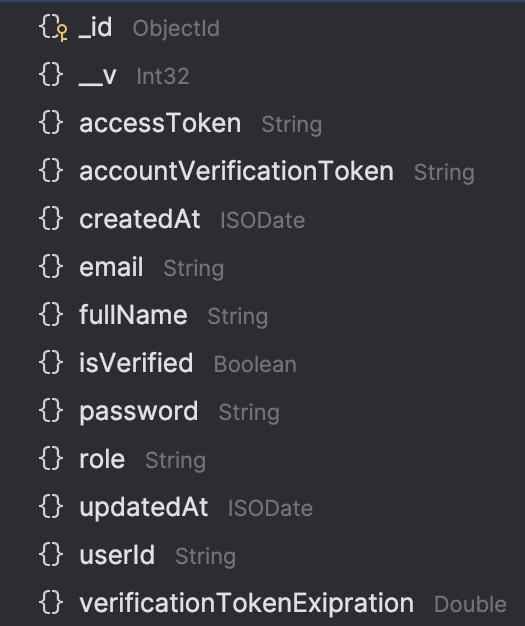
\includegraphics{account-schema.png}
  \caption*{Account Schema}
  \label{fig:acc-shcema}
\end{figure}

\subsubsection{User Schema (\texttt{users})}
Represents user profiles.
\begin{description}
  \item[\texttt{email}, \texttt{fullName} (\emph{String}, required, unique\textsuperscript{*})]  
    Basic identity fields; email is unique to enforce one profile per account.
  \item[\texttt{description} (\emph{String})]  
    Optional biography or profile summary.
\end{description}
\textsuperscript{*}An index enforces email uniqueness at the database level.

\begin{figure}[H]
  \centering
  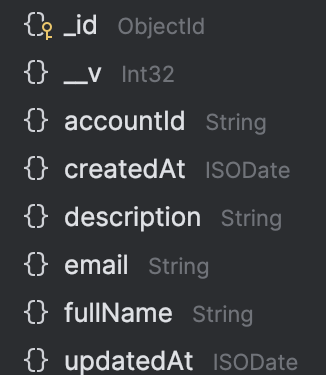
\includegraphics{profile-schema.png}
  \caption*{User Schema}
  \label{fig:profile-schema}
\end{figure}

\subsubsection{Conversation Schema (\texttt{conversations})}
Defines chat groups and direct-message threads.
\begin{description}
  \item[\texttt{participants} (\emph{[ObjectId]}, required)]  
    List of user IDs involved in the conversation.
  \item[\texttt{title}, \texttt{description} (\emph{String})]  
    Optional metadata for group chats or topic summaries.
\end{description}

\begin{figure}[H]
  \centering
  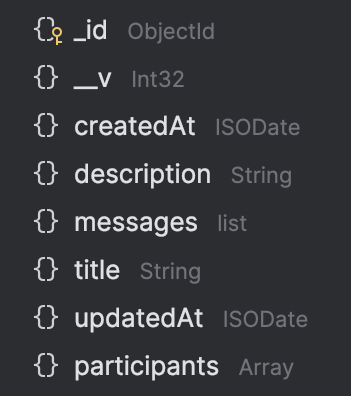
\includegraphics{conversation-schema.png}
  \caption*{Conversation Schema}
  \label{fig:conversation-schema}
\end{figure}

\subsubsection{Message Schema (\texttt{messages})}
Stores individual chat messages within conversations.
\begin{description}
  \item[\texttt{createdBy} (\emph{ObjectId}, required)]  
    Authoring user`s ID.
  \item[\texttt{conversationId} (\emph{ObjectId}, required)]  
    Parent conversation reference.
  \item[\texttt{text} (\emph{String}, required)]  
    Message content.
  \item[\texttt{seenBy} (\emph{[ObjectId]}, default: \texttt{[]})]  
    IDs of users who have read the message.
  \item[\texttt{reactions} (\emph{[String]}, default: \texttt{[]})]  
    Emoji or reaction identifiers attached by users.
  \item[\texttt{isDeleted}, \texttt{isEdited} (\emph{Boolean}, default: \texttt{false})]  
    Flags for deletion and edit status.
\end{description}

\begin{figure}[H]
  \centering
  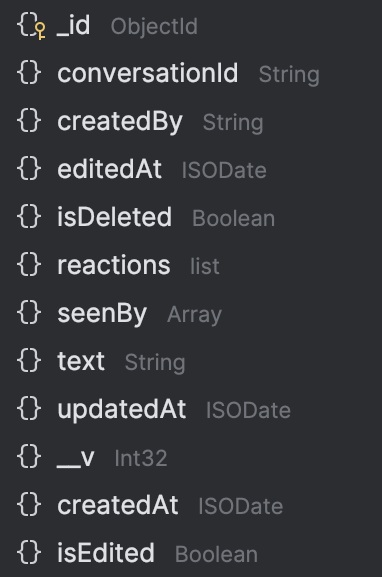
\includegraphics{message-schema.png}
  \caption*{Message Schema}
  \label{fig:message-schema}
\end{figure}

\subsubsection{Notification Schema (\texttt{notifications})}
Captures system alerts and user-to-user notifications.
\begin{description}
  \item[\texttt{sendTo} (\emph{[ObjectId]}, required)]  
    Recipients of the notification.
  \item[\texttt{topic} (\emph{String}, enum)]  
    Notification category (e.g.\ new message, new reaction to message).
  \item[\texttt{data} (\emph{Object})]  
    Payload containing contextual information (e.g.\ IDs, message previews).
  \item[\texttt{isSeen} (\emph{Boolean}, default: \texttt{false})]  
    Read/unread flag.
\end{description}

\begin{figure}[H]
  \centering
  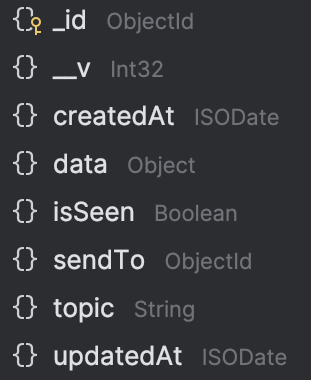
\includegraphics{notification-schema.png}
  \caption*{Notification Schema}
  \label{fig:notification-schema}
\end{figure}

\subsubsection{File Metadata Schema (\texttt{files})}
Models additional data for uploaded files.
\begin{description}
  \item [\texttt{name} (\emph{String}, required)]  
    Original file name as provided by the user. 
  \item [\texttt{description} (\emph{String})]  
    Optional description or caption for the file.
  \item [\texttt{size} (\emph{Number}, required)]  
    Size of the file in bytes.
  \item [\texttt{mimeType} (\emph{String}, required)]  
    MIME type of the file (e.g., image/jpeg, application/pdf).
  \item [\texttt{fileURL} (\emph{String}, required)]  
    URL pointing to the file in the S3-compatible object storage.
  \item [\texttt{uploadedBy} (\emph{ObjectId}, required)]
    Reference to the user who uploaded the file.
\end{description}

\begin{figure}[H]
  \centering
  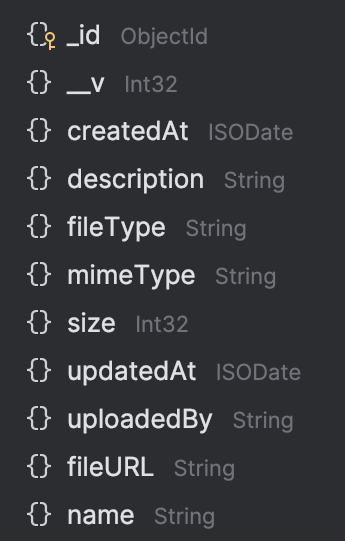
\includegraphics{file-schema.png}
  \caption*{File Metadata Schema}
  \label{fig:file-schema}
\end{figure}

\subsection{Indexes and Performance}

To ensure low-latency queries and maintain data integrity, we define several indexes across our collections and deploy MongoDB in a clustered, highly available configuration.

\paragraph{Indexes}
\begin{itemize}
  \item \textbf{Unique Indexes}
    \begin{itemize}
      \item \texttt{accounts.email}: enforces one account per email address.
      \item \texttt{users.email}: guarantees unique user profiles.
    \end{itemize}

  \item \textbf{Single-Field Indexes}
    \begin{itemize}
      \item \texttt{messages.conversationId}: accelerates retrieval of all messages in a conversation.
      \item \texttt{notifications.sendTo}: speeds up lookup of unread notifications for a given user.
    \end{itemize}

  \item \textbf{Compound Indexes}
    \begin{itemize}
      \item \texttt{messages.{conversationId, createdAt}}: supports paginated fetches of recent messages by conversation.
      \item \texttt{conversations.participants}: optimizes queries for all conversations a user participates in.
    \end{itemize}

  \item \textbf{TTL Indexes}
    \begin{itemize}
      \item \texttt{accounts.verificationTokenExpiration}: automatically removes stale verification tokens.
      \item \texttt{accounts.resetTokenExpiration}: expires old password-reset tokens without manual cleanup.
    \end{itemize}
\end{itemize}

% \paragraph{Sharding and Replication}
% \begin{itemize}
%   \item \textbf{Replica Sets:}  
%     Each MongoDB deployment runs as a three-node replica set, providing automatic failover and durable write acknowledgment with \texttt{w: "majority"} write concern.

%   \item \textbf{Sharding:}  
%     For collections with high write volume (notably \texttt{messages} and \texttt{notifications}), we use a hashed shard key on \texttt{conversationId} or \texttt{sendTo} respectively.  This distributes data evenly across shards and prevents hotspotting.

%   \item \textbf{Read/Write Scaling:}  
%     Secondary replicas handle read traffic for analytics and notification polling (configured with appropriate read preferences), while primaries manage transactional writes and TTL‐driven deletions.

%   \item \textbf{Monitoring and Tuning:}  
%     We leverage MongoDB’s built‐in performance advisor and metrics exporters (via Prometheus) to detect slow queries, adjust index definitions, and scale shards dynamically based on CPU, memory, and disk I/O.
% \end{itemize}

\section{Testing strategies}

Robust automated testing is essential to maintain code quality, prevent regressions, and accelerate feature development.  In \emph{Cloud Class}, we leverage Jest—integrated with NestJS’s testing utilities—to implement a suite of unit tests covering all critical business logic, with a focus on authentication, file uploads, and message handling.

\subsection{Framework and Configuration}

\begin{itemize}
  \item \textbf{Jest}  
    \begin{itemize}
      \item Default test runner for NestJS projects; supports mocks, spies, snapshot testing, and coverage reporting out of the box.
      \item Configured via \texttt{jest.config.ts} to transform TypeScript, collect coverage, and ignore compiled output directories.
    \end{itemize}

  \item \textbf{NestJS Testing Module}  
    \begin{itemize}
      \item Uses \texttt{Test.createTestingModule()} to instantiate a lightweight application context.
      \item Allows overriding providers with mocked implementations or in-memory substitutes (e.g.\ in-memory MongoDB) for isolation.
    \end{itemize}
\end{itemize}

\subsection{Unit Tests}

I prioritized unit tests for core functionalities, ensuring that key features behave correctly under both normal and error conditions.

\begin{itemize}
  \item \textbf{Authentication}
    \begin{itemize}
      \item \texttt{signing up}: verifies password hashing, user creation, and error on duplicate email.
      \item \texttt{validating users}: checks credential validation logic.
      \item Edge cases: invalid credentials, expired tokens, and role-based access assertions.
    \end{itemize}

  \item \textbf{File Uploads}
    \begin{itemize}
      \item \texttt{upload file}: tests file-type validation, size limits, and interaction with MinIO/S3 API (mocked).
      \item Error scenarios: unsupported formats, storage failures, and retry logic.
    \end{itemize}

  \item \textbf{Messages}
    \begin{itemize}
      \item \texttt{create message}: validates conversation existence and correct document shape.
      \item \texttt{find by conversations}: tests pagination, sorting by timestamp, and filtering out deleted messages.
      \item Mocking of Mongoose Model methods (\texttt{save()}, \texttt{find()}, \texttt{lean()}).
    \end{itemize}
\end{itemize}

Each test file is co-located with its implementation in a \texttt{*.spec.ts} file.  I aimed for at least 80\% coverage on each core of the functionalities, using Jest`s coverage report as a way to monitor it.

\section{Scalability and Performance Considerations}

One of the foremost advantages of a microservice architecture is the ability to scale individual services independently, based on their specific resource demands.  In \emph{Cloud Class}, each of the eight microservices—such as Authentication, WebSocket Server, Uploader, and Notification—can be deployed in its own container and allocated CPU, memory, and I/O budgets that precisely match its workload.  During periods of high messaging activity, for example, the WebSocket Server can be horizontally scaled out to multiple replicas without affecting unrelated services like Uploader or Mailer.  Conversely, when file-upload traffic subsides, the Upload Server replicas can be scaled back to conserve cluster resources and reduce cost.

Dynamic scaling is typically managed through Kubernetes` Horizontal Pod Autoscaler (HPA), which adjusts the number of running pods for each service in response to real-time metrics (CPU utilization, memory usage, or custom application-level metrics like request latency).  By setting sensible targets and thresholds, the system maintains consistent performance under fluctuating load while avoiding overprovisioning.  This elasticity ensures that end-users experience low latency and high throughput—even during peak usage—while keeping infrastructure spend proportional to actual demand.

Beyond pure scaling, microservices also improve fault isolation and deployment agility, both of which contribute to overall performance resilience:

\begin{itemize}
  \item \textbf{Fault Isolation:}  A failure or performance degradation in one service (e.g.\ a heavy file upload in the Uploader Server) does not directly impact the availability or responsiveness of other services.
  \item \textbf{Independent Deployment:}  Each service can be updated, rolled back, or redeployed without requiring a full system outage.  This reduces planned downtime and allows performance optimizations to be rolled out rapidly.
  \item \textbf{Resource Specialization:}  Services with very different I/O patterns—such as compute-heavy data aggregation versus I/O-bound file transfers—can be placed on node pools with hardware tailored to their needs (e.g.\ SSD-backed nodes for storage services, high-CPU nodes for processing).
\end{itemize}

Finally, horizontal scaling and service isolation simplify capacity planning and permit near-linear performance gains: doubling the number of replicas for a stateless service generally doubles its throughput, up to the limits of downstream dependencies (such as the database).  To maximize this benefit, this application also employs deployment best practices such as:

\begin{itemize}
  \item \textbf{Caching Layers:} Introducing in-memory caches (e.g.\ Redis) at strategic service boundaries to offload read-heavy operations and reduce latency.
  \item \textbf{Asynchronous Processing:} Offloading non-critical tasks (notifications) or resource intensive tasks (sending emails, file uploads) to message queues and background workers, smoothing out traffic spikes and decoupling end-user interactions from longer-running processes.
\end{itemize}

Together, these architectural patterns ensure that \emph{Cloud Class} can meet demanding performance requirements today while remaining flexible enough to grow with future user populations and feature sets.
